\newcommand{\specname}{SBCF}
\newcommand{\status}{Beta}
\newcommand{\ecn}{NA}
\newcommand{\revdate}{2013-03-16}
\newcommand{\rev}{000}
\newcommand{\relay}{PB2}
\newcommand{\boil}{PB3}
\newcommand{\led}{PB5}
\newcommand{\wfo}{PB4}
\newcommand{\duty}{PC0}
\newcommand{\probe}{PC1}
\newcommand{\temp}{PC2}
\newcommand{\fast}{PB6}
\newcommand{\faster}{PB7}
\newcommand{\fastest}{PB1}
\newcommand{\delay}{PB0}
\newcommand{\pwma}{PB6}
\newcommand{\pwmb}{PB7}

\documentclass[dvips,12pt]{article}
\renewcommand{\contentsname}{3. Index} 

\usepackage{amsmath}
%\usepackage{program}
\usepackage{a4,color,graphics,palatino,fancyhdr}
\usepackage{lastpage}
\usepackage{fancyhdr}
\usepackage{changepage}% http://ctan.org/pkg/changepage
\usepackage{graphicx}
\usepackage{float}

\floatstyle{ruled}
\newfloat{program}{thp}{lop}
\floatname{program}{Source Code}

\setlength{\headheight}{15pt}

\setcounter{secnumdepth}{1}
\setcounter{tocdepth}{1}

\lhead{\specname}
\rhead{rev.\  \rev} 
\chead{\revdate}
\cfoot{\footnotesize Page\ \thepage\ of \pageref{LastPage}}
\pagestyle{fancy}
\title{Simple Brew Control Firmware}

\author{chaz}

\begin{document}

\frenchspacing


\section{Purpose}
Documentation for Simple Brew Control Firmware, which is a microcontroller program that can be configured as thermostat, boil
controller, kegerator thermostat, or fermentation controller. 

\tableofcontents
\listoffigures

\section{Objective}

Temperature control and PWM control of heating elements is a common need in beer brewing and sous vide. This is a simple
microcontroller firmware that can fulfil these roles and possibly replace expensive special-purpose PID controllers and temperature controls. The firmware also functions as a basic PWM generator and should be useful for other temperature control applications that need selectable open-loop control as well as closed-loop thermostatic control in the same unit. 

\section{Microcontroller hardware}

The microcontroller used is an ATMEGA328 8-bit AVR\textcopyright\ microcontroller which is widely available for about 3
USFRN in convenient packages. It was selected for its availability in my toolbox. The firmware would run on other AVR
microcontrollers with minimal modification. The microcontroller is powered by 5V and runs at 1MHz, which is how it's
configured out-of-the-box.  No external crystal is needed, just apply 5V on the Vcc pin and
pull up RESET (refer to
figure \ref{fig:uc}). Note that if you use a 5V cell-phone power supply, you don't need
any voltage regulator.

Flashing this firmware to the microcontroller will require an in-system-programmer such as the AVRISPV2 or USBTinyISP.
Instructions on programming AVR microcontrollers is outside the scope of this document. All the cool kids are using
Arduino nowadays, and you may be able to pretend this is an Arduino program and try to flash it with the Arduino IDE and
it may Just Work. You are on your own on the Arduino front. If you ask nicely, I may be able to program one for you or
send you a programmed chip for a nominal fee.


\section{Configuration Possibilities}

The firmware is very flexible. It can be a PWM generator, thermostat, or full-featured brew controller. You can make an increasingly featureful system by hooking up more hardware. 

\subsection{PWM}
Simply hook up two resistors to the BOIL analog input (\duty) as a voltage divider (figure \ref{fig:vdiv}). The system
will then toggle the relay output \relay{} at a duty cycle proportional to the voltage applied. Refer to table
\ref{fig:resistors} and figure \ref{fig:vdiv} for resistor values. In this mode you have a
simple pulse-width-modulation (PWM) generator that is similar to all the 555-timer-based PWM circuits out there. If all you need to do is knock down a heating element's wattage, this might be all you need. 

If you want variable output, just use a potentiometer instead of 2 resistors--then, the
firmware is a varible PWM generator. You could use the analog input to set the duty cycle with
some other system, if you so desire.

\subsection{Boil Override Switches} 
You can add more options to your PWM controller by hooking two switches (or one 3-position ``center-off'' switch) from
ground the BOIL and WFO digital inputs on PB5 and PB3, respectively. This is the same as above--it's still a PWM
generator--only now there are 2 additional options: WFO (Water Fully On) and BOIL (fixed 60\% by default).  Turning these
switches on overrides the main PWM setting on \duty. This allows you to get your knob set where you want it, but still
have an easy override to 100\% and (by default) 60\%. This could be a good configuration for a hot-wire foam-cutter. 

\subsection{Thermostat Functionality} 
You can use analog inputs \probe{} and \temp{} to create a thermostat. Input \probe{} reads the temperature sensor, and
\temp{} reads a temperature setpoint knob. In this mode, the firmware turns the output on only if the temperature
(voltage on \probe) is below temperature setpoint (voltage on \temp). If you want a ``cool'' mode thermostat, such as for
a kegerator, just swap the \temp{} and \probe{} inputs. Note that once the thermostat commands the output ON, the duty
cycle of the output is still whatever is set by \duty. You need to connect \duty{} to +5V, resistors, or a pot depending
if you want the output \% to be full, partial, or adjustable. For a kegerator, you definitely want to pull \duty{} up to
5V. Refer to figures \ref{fig:max}.

\section{How I use it}

For brewing, I use the full configuration. I use the thermostat functionality with the power knob turned all the
way up to heat my mash water to strike temperature while I do something
else. After I dough-in my grain, I again use the thermostat mode to
maintain mash temperatures, only I turn the knob down to about 30\% for more gentle heat to 
prevent scorching. After the mash, I disconnect the temp probe (you don't need to, though) and kick the
switch to WFO until I have a good boil, then kick it to BOIL for a very
consistent and repeatable boil with a predictable rate of boil-off. 

\section{Stuff you didn't want to know}

The PWM duty cycle is about 1Hz by default. This is good for most brewing/cooking applications driven by mains
electricity. To increase it to 4Hz, connect \fast{} to ground. To increase it to 240Hz (maybe for hot-wire cutting or
dimming LEDs), connect \faster{} to ground. For 2kHz, which is good for small DC motors, connect \fastest{} to ground.
However, the 2kHz setting may decrease accuracy of analog readings.

Kegerator thermostats typically have a ``compressor delay'' feature  to protect the compressor from fast-cycling. To
enable a compressor delay feature, connect \delay{} to ground.

\section{Perhipheral hardware options}

\renewcommand{\arraystretch}{1.4}% adjust hline heights for prettiness
\begin{figure}[h]
\centering
\begin{tabular}{|c|c|c|c|}
\hline
Input Item&AVR Pin&Voltage details& Function notes\\
\hline
Boil Switch&\boil&GND=BOIL&Override duty cycle for boiling \\
\hline
WFO Switch&\wfo&GND=WFO&Override duty cycle to 100\% \\
\hline
Temp probe&\probe&0V-5V analog in&LM335 \\
\hline
BOIL pot&\duty&0V-5V analog in&Heating element power\\
\hline
TEMP pot&\temp&0V-5V analog in&Temp setpoint\\
\hline
PWM select A&\pwma&GND or N.C.&per figure \ref{fig:freq}\\
\hline
PWM select B&\pwmb&GND or N.C.&per figure \ref{fig:freq}\\
\hline
Compressor delay&\delay&GND or N.C.&GND=delay enabled\\
\hline
\end{tabular}
\caption{Table Of Inputs}
\label{fig:inputs}
\end{figure}

\renewcommand{\arraystretch}{1.4}% adjust hline heights for prettiness
\begin{figure}[h]
\centering
\begin{tabular}{|c|c|c|c|}
\hline
Output Item&AVR Pin&Voltage details& Function notes\\
\hline
Blinkenled&\led&LED+resistor&Blinks\\
\hline
SSR&\relay&Hook to SSR&5V=heater on\\
\hline
\end{tabular}
\caption{Table Of Outputs}
\label{fig:outputs}
\end{figure}

\renewcommand{\arraystretch}{1.4}% adjust hline heights for prettiness
\begin{figure}[h]
\centering
\begin{tabular}{|c|c|c|c|}
\hline
R1&R2&\duty Voltage&Duty Cycle\\
\hline
0&$\infty$&5V&100\%\\
\hline
1000&4000&4V&80\%\\
\hline
2200&2200&2.5V&50\%\\
\hline
4000&1000&1V&20\%\\
\hline
$\infty$&0&0V&0\%\\
\hline
\end{tabular}
\caption{Resistor values for various fixed PWM duty cycles}
\label{fig:resistors}
\end{figure}

\renewcommand{\arraystretch}{1.4}% adjust hline heights for prettiness
\begin{figure}[h]
\centering
\begin{tabular}{|c|c|c|c|}
\hline
PB6&PB7&PWM frequency\\
\hline
na&na&1Hz\\
\hline
GND&na&4Hz\\
\hline
na&GND&240Hz\\
\hline
GND&GND&2000Hz\\
\hline
\end{tabular}
\caption{Pin settings for changing PWM frequency}
\label{fig:freq}
\end{figure}


\begin{figure}[h]
    \begin{centering}
    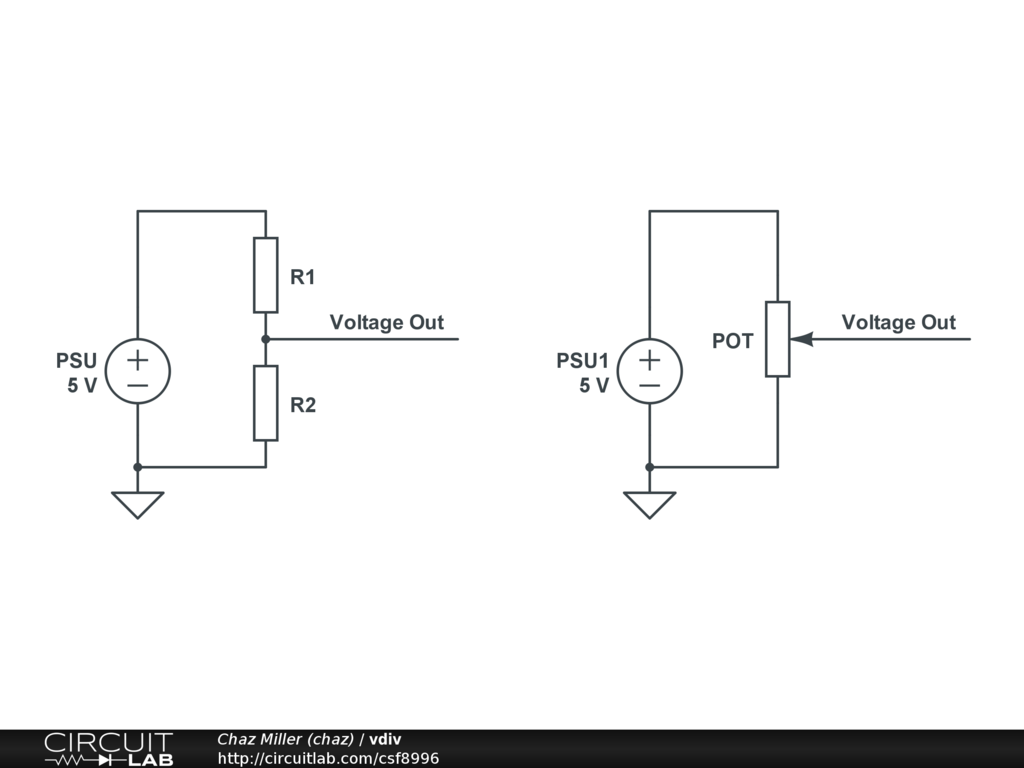
\includegraphics[width=0.8\textwidth]{vdiv}
    \caption{Fixed (left) and variable (right) voltage dividers}
    \label{fig:vdiv}
    \end{centering}
\end{figure}

\begin{figure}[h]
    \begin{centering}
    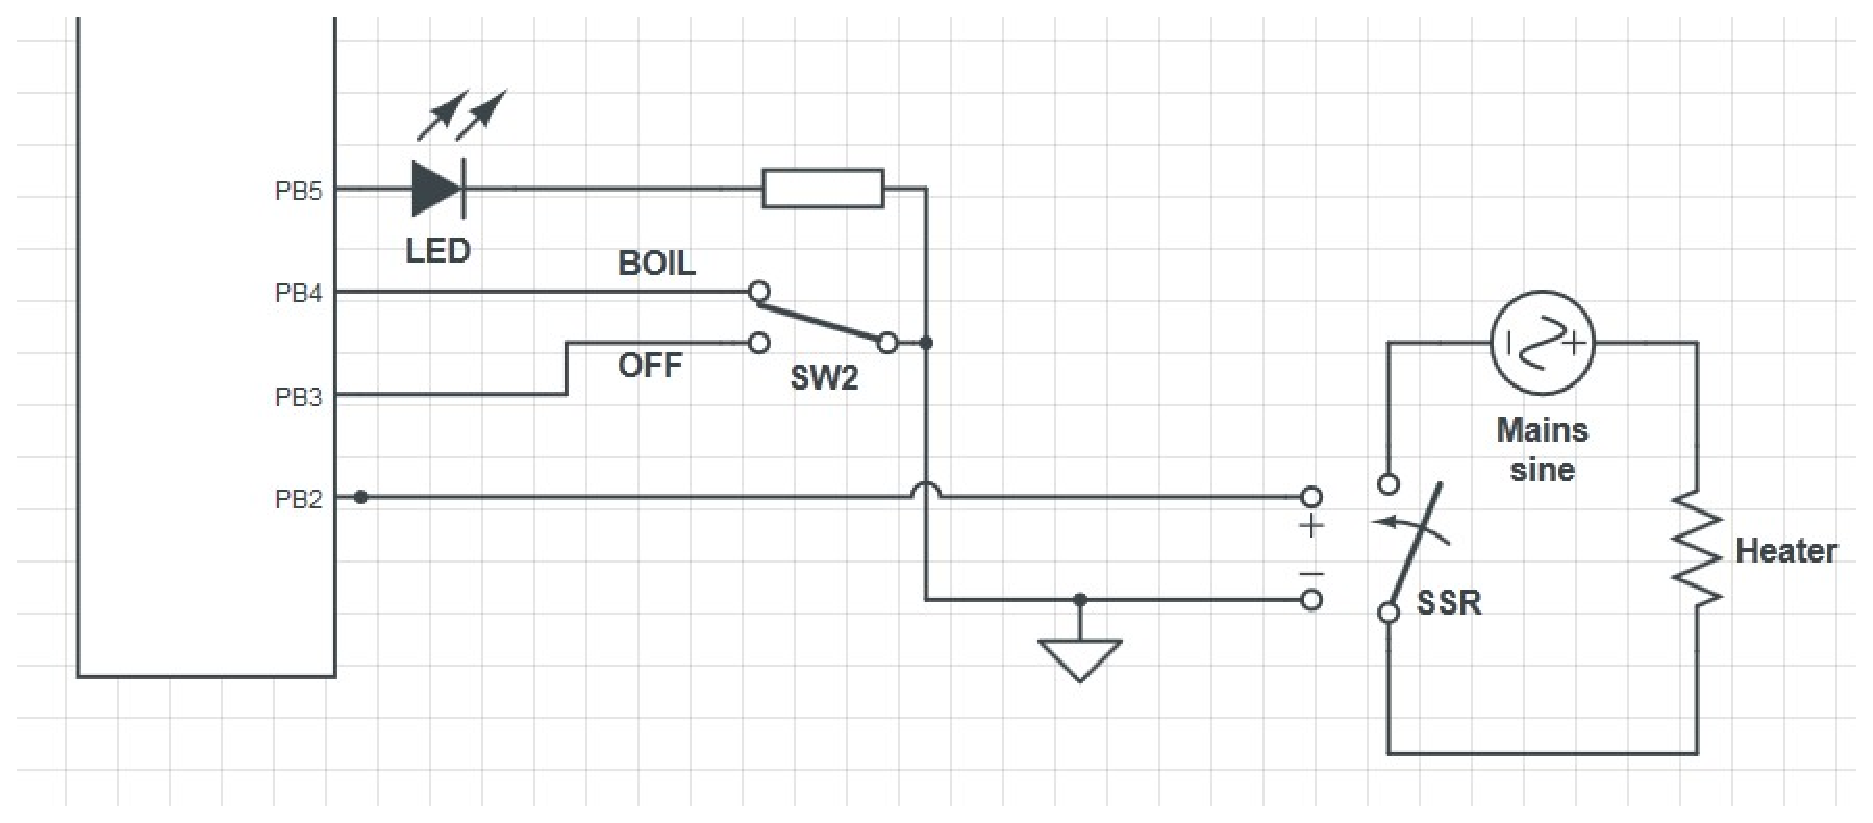
\includegraphics[width=0.8\textwidth]{min}
    \caption{Example minimal system for heating element control}
    \label{fig:min}
    \end{centering}
\end{figure}


\begin{figure}[h]
    \begin{centering}
    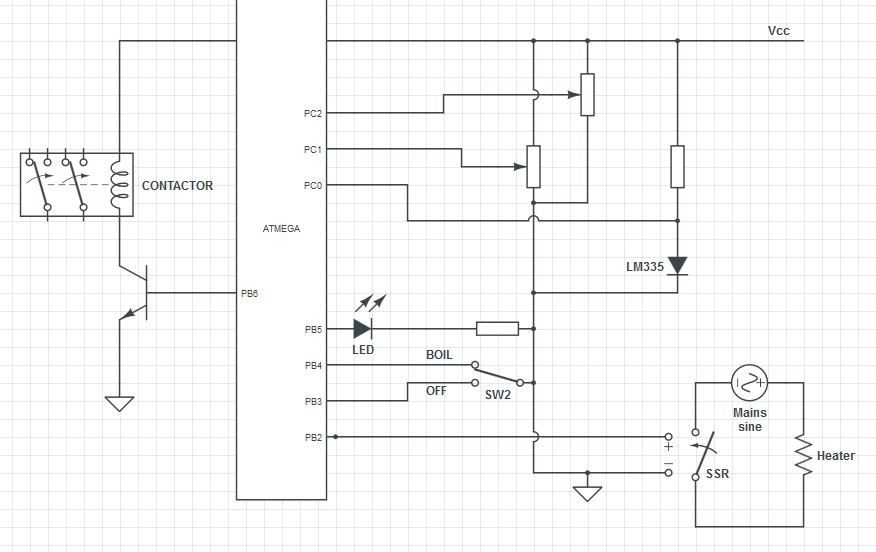
\includegraphics[width=0.8\textwidth]{max}
    \caption{Example complete system with thermostat} 
    \label{fig:max}
    \end{centering}
\end{figure}

\begin{figure}[h]
    \begin{centering}
    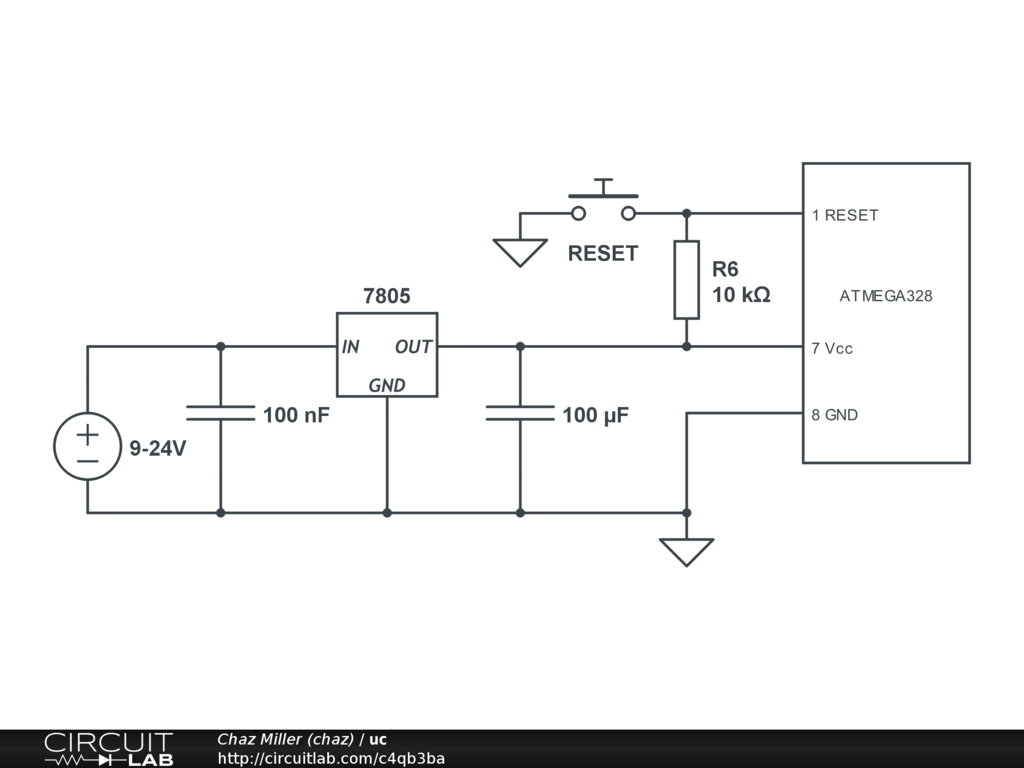
\includegraphics[width=0.8\textwidth]{uc}
    \caption{Microcontroller connections. If clean 5V power (e.g. USB) the LM7805 is unneeded.} 
    \label{fig:uc}
    \end{centering}
\end{figure}
\begin{figure}[h]
    \begin{centering}
    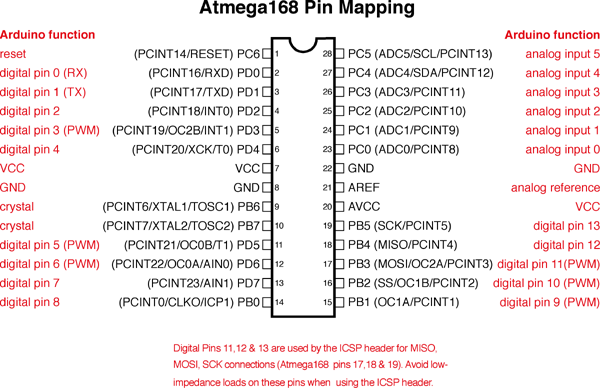
\includegraphics[width=0.8\textwidth]{pins}
    \caption{Pinout for ATMEGA168/328 DIP package} 
    \label{fig:pins}
    \end{centering}
\end{figure}




\centering
\vspace{2cm}
\appendix

\end{document}

